\documentclass[10pt]{article}
\usepackage[margin=.8in]{geometry}
\usepackage[T1]{fontenc}\usepackage{lmodern}
\usepackage{booktabs,array,longtable,tabularx,enumitem,hyperref,tikz}
\usetikzlibrary{arrows.meta,positioning}
\hypersetup{hidelinks}
\setlist[itemize]{leftmargin=1.8em,itemsep=.55em,topsep=.55em,parsep=.15em}
\setlist[enumerate]{leftmargin=2.2em,itemsep=.7em,topsep=.55em,parsep=.2em}
\setlength{\emergencystretch}{1.5em}
\newcommand{\code}[1]{\texttt{#1}}
\title{TriAlign Engineering and Delivery Plan\\\large Evaluating and Improving Clinical-Meaning Distances in Trial Eligibility Embeddings}
\author{Jonathan Ma \and Jiatong Gao}
\date{Revised October 28, 2026}

\begin{document}
\maketitle\tableofcontents

\section{Objective and Clinical Significance}
Eligibility criteria define the population to which a trial applies, but similar wording does not guarantee similar clinical meaning. ``Age $\geq18$'' and ``age $<18$'' are lexically close yet disjoint. Negation, thresholds, units, timing, repetition, exceptions, treatment history, and Boolean scope create similar failures.

TriAlign is downstream of Modern AutoCrit. Modern AutoCrit converts protocol prose into reviewed atomic records with structured fields, identifiers, context, and source evidence. TriAlign will retrieve comparable criteria across protocols, predict an explicit relationship (equivalent, one more restrictive, overlapping, disjoint, related but not comparable, unrelated, or ambiguous), explain the evidence, and route exact, embedding-based, or contextual reasoning through an auditable agent. Accepted pair labels will improve a dense eligibility encoder.

The practical user is a clinical team comparing a current rule with historical trials. TriAlign is protocol-comparison decision support, not automated patient screening or proof of transportability.

\subsection*{Research questions}
\begin{enumerate}
\item Which clinical phenomena cause general and biomedical embeddings to produce false-high or false-low similarity?
\item Does training on reviewed positives, ordinary negatives, hard negatives, and ordered anchors improve retrieval and relationship prediction on held-out trial families?
\item Does agentic routing improve evidence support, calibration, and reviewer efficiency over an LLM-only judge or fixed tool chain?
\end{enumerate}

\section{Modern AutoCrit Primer and Data Handoff}
\subsection{What the upstream system does}
Modern AutoCrit is the upstream data-production system; TriAlign does not replace it. Its workflow is:
\begin{itemize}
\item accept an NCT identifier, protocol text, or protocol PDF;
\item locate the eligibility section and separate inclusion from exclusion rules;
\item split eligibility prose into atomic, comparison-ready criteria;
\item preserve the original criterion, parent statement, surrounding context, and protocol provenance;
\item add domain/entity, comparator, value, unit, interval, negation, timing, repetition, qualifiers, and Boolean links; and
\item record stable identifiers, source versions, validation findings, extraction confidence, and human-review status.
\end{itemize}
These records are inspected and corrected before they enter TriAlign.

For example, ``blood pressure $>145/95$ on two occasions within three months'' should retain the blood-pressure entity, comparator and compound value, the repetition count, the three-month temporal window, and its inclusion/exclusion role. Flattening it to a sentence embedding would hide the exact features needed to decide whether another criterion is equivalent, broader, narrower, or disjoint.

\subsection{Terminology normalization}
Modern AutoCrit also performs terminology normalization. It maps abbreviations, spelling variants, aliases, and clinically equivalent surface forms to a canonical entity while preserving the raw wording. Examples include expanded/abbreviated disease names, laboratory aliases, and oncology terminology. Normalization supports candidate retrieval across trials, but it must not erase clinically meaningful distinctions such as disease stage, severity, anatomical site, measurement method, or treatment context. Every normalized term therefore remains traceable to its source text, normalization rule/library version, and any human correction. TriAlign will use both the canonical fields and raw/context text, and will explicitly test whether normalization creates false merges or fails to merge true synonyms.

\subsection{Current corpus and review state}
The source corpus contains 100 public trials: 50 oncology and 50 cardiovascular studies. The initial Modern AutoCrit export contained 3,145 candidate criteria with NCT and source versions; parent and atomic text; structured comparison and semantic fields; validation findings; and review status. Human correction can split a compound source row into multiple atomic rows, so reviewed-workbook counts need not equal the original candidate count.

Criterion review is in progress. By the October 20 presentation, approximately 2,900 cases had been human-reviewed and roughly 600 uncertain or difficult cases remained. Review consists of:
\begin{itemize}
\item correcting segmentation, structured fields, and clinical meaning;
\item creating linked rows for genuinely compound criteria;
\item preserving parent statements and source evidence;
\item marking unresolved ambiguity rather than guessing; and
\item admitting only accepted or corrected, validation-passing records to the frozen corpus.
\end{itemize}
The workbook, validated export, manifest, schema, normalization-library version, Git revision, and fingerprint will be archived together.

There are two distinct reviews. \emph{Criterion review} checks whether Modern AutoCrit faithfully represented one protocol rule. Later, \emph{pair review} compares two already-reviewed criteria and assigns the TriAlign relationship label, direction, supporting evidence, and ambiguity status. Criterion approval is not automatically a pair label. If full review is incomplete by November 17, a versioned development subset will be reported honestly and kept separate from the final test set.

\subsection{Minimum handoff vocabulary}
The core terms used throughout the project are:
\begin{longtable}{p{.24\linewidth}p{.68\linewidth}}\toprule
Term & Meaning in this project\\\midrule
Source criterion & Exact protocol wording used as evidence; never silently rewritten.\\
Parent statement & Larger sentence/list item from which one or more atomic rows were derived.\\
Atomic criterion & One comparison-ready eligibility rule. Compounds may produce linked atomic rows.\\
Canonical entity & Normalized clinical concept used to find candidate matches across wording variants.\\
Structured constraint & Comparator/value/unit plus negation, timing, repetition, qualifier, and Boolean scope when present.\\
Criterion review & Human verification of extraction and normalization for one row.\\
Pair review & Human judgment of the clinical relationship between two reviewed rows.\\
Ready record & Source-grounded, validation-passing, human-accepted/corrected record eligible for TriAlign.\\\bottomrule
\end{longtable}

\section{AI and Agent Workflow}
\begin{figure}[ht]\centering
\resizebox{\textwidth}{!}{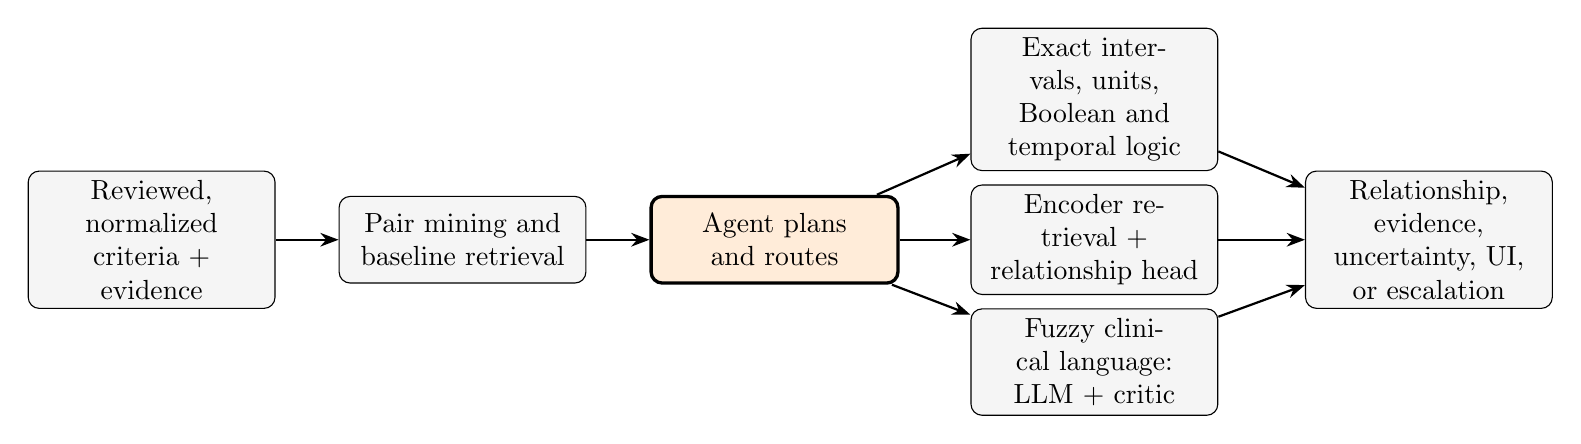
\begin{tikzpicture}[node distance=8mm,box/.style={draw,rounded corners,fill=gray!8,text width=29mm,minimum height=11mm,align=center},agent/.style={box,fill=orange!15,very thick},arr/.style={-{Stealth},thick}]
\node[box](data){Reviewed, normalized\\criteria + evidence};
\node[box,right=of data](pairs){Pair mining and\\baseline retrieval};
\node[agent,right=of pairs](route){Agent plans\\and routes};
\node[box,above right=3mm and 9mm of route](exact){Exact intervals, units,\\Boolean and temporal logic};
\node[box,right=9mm of route](embed){Encoder retrieval +\\relationship head};
\node[box,below right=3mm and 9mm of route](llm){Fuzzy clinical language:\\LLM + critic};
\node[box,right=11mm of embed](out){Relationship, evidence,\\uncertainty, UI,\\or escalation};
\draw[arr](data)--(pairs);\draw[arr](pairs)--(route);\draw[arr](route)--(exact);\draw[arr](route)--(embed);\draw[arr](route)--(llm);\draw[arr](exact)--(out);\draw[arr](embed)--(out);\draw[arr](llm)--(out);
\end{tikzpicture}}\caption{TriAlign runtime. Routing, rather than calling every tool in sequence, is the agentic contribution.}
\end{figure}

Before routing, a terminology-aware retrieval layer uses canonical entities and aliases to propose candidates while retaining the raw wording and surrounding context. The deterministic route handles compatible intervals, units, explicit negation, Boolean presence, and simple timing. The encoder performs scalable cross-trial retrieval. The contextual route handles exceptions, severity, history, incompatible measurements, and ambiguous scope. Routes may be combined to identify conflicts. Every result retains source excerpts, normalized and raw field differences, model/tool/normalization versions, uncertainty, escalation, and human correction. Training occurs offline; runtime weights are frozen.

\section{Models and Recent Eligibility Systems}
\subsection{Direct, matched-task baselines}
\begin{longtable}{p{.22\linewidth}p{.31\linewidth}p{.38\linewidth}}\toprule
System & Implementation & Purpose\\\midrule
Lexical & TF--IDF + cosine & Transparent word-overlap reference.\\
General encoder & \code{all-mpnet-base-v2} & Frozen Hugging Face semantic baseline.\\
Biomedical encoder & \code{FremyCompany/BioLORD-2023} & Biomedical representation baseline.\\
CReSE-informed & Published eligibility representation method where artifacts permit \cite{crese} & Closest criterion-representation comparator.\\
LLM-only judge & One schema-constrained pair prompt & Contextual reasoning without routing.\\
Fixed chain & Exact tools, encoder, and LLM always called & Separates routing from composition.\\
TriAlign & Fine-tuned MPNet, directional head, exact tools, critic, router & Full system.\\\bottomrule
\end{longtable}

The relationship head is separate because cosine is symmetric and cannot state that A is more restrictive than B.

\subsection{Agentic and adjacent comparisons}
\begin{itemize}
\item \textbf{TrialGPT} performs trial retrieval, patient--criterion judgments, and ranking \cite{trialgpt}; we will adapt its evidence-and-judgment pattern to common criterion pairs.
\item \textbf{EligMeta} combines LLM parsing and deterministic execution for eligibility-aware evidence synthesis \cite{eligmeta}; we compare compatible alignment outputs, not meta-analysis performance.
\item \textbf{SatIR} formalizes patient/trial constraints with SMT and relational algebra \cite{satir}; it motivates TriAlign's exact route.
\item \textbf{VERDICT} combines LLM translation with SMT/MaxSMT and evaluates grounded rationales, consistency, pivotal conditions, and counterfactual self-faithfulness \cite{verdict}; TriAlign will adopt compatible consistency tests.
\item \textbf{EC-RAFT} generates eligibility criteria using retrieval-augmented fine-tuning \cite{ecraft}; it informs future authoring applications but is not a direct comparison baseline.
\end{itemize}
These systems solve different primary tasks. We will use (1) matched-case comparisons of labels, evidence, abstention, latency, and cost where outputs align, and (2) design/failure-mode comparisons otherwise. We will not claim one unqualified leaderboard.

\section{Benchmark and Evaluation}
\subsection{Definition of a criterion pair}
A \emph{criterion pair} is an ordered comparison between two individually reviewed eligibility criteria, criterion A and criterion B, normally drawn from different protocols. A pair is not merely two text strings. Its record preserves both criterion and trial identifiers, raw text, parent statements, surrounding context, structured fields, source links, sampling method, and any baseline retrieval score. The order matters for directional relationships: if A is more restrictive than B, reversing the pair changes the label to B more restrictive. Symmetric labels such as equivalent, disjoint, unrelated, and ambiguous do not change when the order is reversed.

JM owns pair definition, candidate selection, human labeling, adjudication, and validation. The pair labels are:
\begin{itemize}
\item \textbf{Equivalent:} both criteria define the same operational eligibility rule despite possible wording differences.
\item \textbf{A more restrictive:} everyone satisfying A should satisfy B, but B permits additional participants.
\item \textbf{B more restrictive:} everyone satisfying B should satisfy A, but A permits additional participants.
\item \textbf{Partial overlap:} the criteria share some eligible population, but neither contains the other.
\item \textbf{Contradictory or disjoint:} no participant can satisfy both criteria under the stated interpretation.
\item \textbf{Related but not comparable:} the criteria concern a related concept but do not define an ordered or overlapping population relationship on the available information.
\item \textbf{Unrelated:} the criteria concern different clinical concepts without a meaningful direct comparison.
\item \textbf{Ambiguous:} source context or clinical meaning is insufficient for a defensible relationship judgment.
\end{itemize}

JM will construct the labeling guide, select natural and diagnostic pairs, inspect source evidence, assign labels, record rationale and uncertainty, validate directionality and consistency, and maintain unresolved cases as ambiguous. JG may consume the resulting development pairs to test software, but does not define or validate the gold labels.

Trials are split by family before pairing; amendments, templates, duplicates, and constructed variants remain together. Test labels are unavailable to training, prompting, model selection, or agent retrieval. Pairs include natural neighbors from multiple encoders, random controls, equivalent paraphrases, broader/narrower rules, thresholds, intervals, negation, timing, repetition, exceptions, compounds, and marked constructed challenges.

\begin{longtable}{p{.29\linewidth}p{.63\linewidth}}\toprule
Question & Measures\\\midrule
Retrieval quality & Precision/recall@$k$, reciprocal rank, equivalence retrieval, anchor ordering.\\
Clinical differences & Phenomenon-specific errors; directional macro-F1; input-order consistency.\\
Uncertainty & Calibration, risk--coverage, inappropriate acceptance, abstention/escalation errors.\\
Agent value & LLM-only vs fixed chain vs routing: evidence support, corrections, reviewer time, latency, cost.\\
Component value & Ablate hard negatives, human corrections, exact checks, critic, and targeted sampling; at least three seeds.\\
Uncertainty of results & Paired comparisons and intervals preserving trial-family dependence; natural and constructed cases separate.\\\bottomrule
\end{longtable}
Both positive and negative preliminary/final results are required. Failures include false-high/low similarity, unsupported rationales, routing errors, source-context errors, and necessary abstentions.

\section{Two-Person Division of Work}
\begin{longtable}{p{.17\linewidth}p{.37\linewidth}p{.37\linewidth}}\toprule
& Jonathan Ma & Jiatong Gao\\\midrule
Primary ownership & Frozen criterion corpus; terminology normalization; pair definitions, construction, labeling, adjudication, and validation; trial-family mapping; evaluation data; provenance and packaging. & Implemented and tested TF--IDF, MPNet, and BioLORD baselines; TrialGPT/EligMeta comparison plan; orchestrator, tool interfaces, critic, traces, and agentic workflow.\\
Data and prototype & Freeze development criteria; publish the pair-label guide; create and validate pilot labels; supply development pairs and structured tools. & Run the three baselines on supplied pairs; investigate comparable TrialGPT/EligMeta functions; build the first auditable orchestrator and route trace.\\
Final system and evaluation & Freeze pair benchmark and splits; validate labels/direction/source evidence; define metrics and verify case-level results. & Complete baseline evaluation, external-system adapters where feasible, routing, conflict reconciliation, critic, abstention, and UI-facing agent outputs.\\
Submission package & Complete data/pair manifests, labeling documentation, source evidence, test-case index, and reproducibility package. & Complete baseline and agent code, prompts/configurations, traces, technical tests, and implementation documentation.\\\bottomrule
\end{longtable}

Shared work: review each other's pull requests, agree on the input/output contract between labeled pairs and the agent, inspect representative successes and failures, verify both demonstrations, and report contributions by artifacts and commits. JM remains the authority for pair labels and evaluation-set changes; JG remains the owner of baseline and orchestrator implementation.

\section{Live Demonstration Plan}
Both remaining presentations require a live demonstration, so the UI is a scheduled deliverable rather than a final cosmetic layer. The demonstration should answer one practical question: \emph{given a criterion from a current trial, what comparable historical criteria exist, how do they differ clinically, and why should the user trust or question the result?}

The minimum demonstration flow is:
\begin{enumerate}
\item select a trial and criterion or enter criterion text;
\item display the raw source, normalized Modern AutoCrit representation, and protocol provenance;
\item retrieve comparable criteria across other protocols;
\item show which route the agent selected---exact structured comparison, encoder retrieval, contextual LLM/critic review, or a combination;
\item display relationship, direction, component evidence, uncertainty, and source links side by side;
\item allow the user to accept, correct, or mark the result unresolved, and export the trace.
\end{enumerate}

\subsection{Visualization priorities}
Visualizations are ranked by the combination of clinical usefulness, explanatory value during a demonstration, and implementation feasibility. The dashboard should implement the highest-ranked items first rather than attempting every visualization.

\begin{enumerate}
\item \textbf{Side-by-side constraint comparison --- highest priority.} \emph{Feasibility: high; usefulness: very high.} Show query and candidate fields in aligned rows for entity, comparator, value, unit, interval, negation, timing, repetition, qualifier, Boolean scope, and source. Use restrained colors for matches, clinically meaningful differences, contradictions, and missing information. This view directly explains the final relationship and works for both numerical and textual criteria.

\item \textbf{Numerical interval or coverage plot.} \emph{Feasibility: high; usefulness: very high for numerical cases.} Draw both allowed regions on a shared number line and mark their intersection, containment, or separation. The visualization should be generated from parsed interval endpoints rather than from model scores. It provides the clearest demonstration of why criteria such as age $\geq18$ and age $<18$ may be close in embedding space but clinically disjoint.

\item \textbf{Agent decision trace.} \emph{Feasibility: high; usefulness: very high.} Display the route as a compact flow: input validation, candidate retrieval, exact/encoder/contextual tool selection, tool outputs, conflict reconciliation, critic result, and final decision or escalation. Each node should expand to show the input and output used. This makes the agentic contribution visible and distinguishes routing from a single LLM call.

\item \textbf{Method-agreement panel.} \emph{Feasibility: high; usefulness: high.} Present the result from TF--IDF, the general encoder, biomedical encoder, structured comparator, LLM judge, critic, and final TriAlign decision in one table. Highlight disagreement instead of collapsing it into one unexplained score. Only calibrated model probabilities should be labeled as probabilities; deterministic results should be labeled exact and uncalibrated scores as scores.

\item \textbf{Uncertainty and review indicator.} \emph{Feasibility: medium; usefulness: high once calibration is available.} Report one of three actions---accept, human review recommended, or abstain---alongside calibrated confidence, route, and reason. Until calibration is validated, the UI should show raw scores and an explicit ``not calibrated'' label rather than implying statistical certainty.

\item \textbf{Embedding similarity versus clinical relationship plot.} \emph{Feasibility: medium; usefulness: high for results and error analysis.} Plot baseline cosine similarity on the horizontal axis and the reviewed/TriAlign relationship on the vertical axis or by color. Label false-high and false-low examples. This plot demonstrates the central embedding gap across the benchmark, but it is more useful as a cohort-level results view than as the primary single-pair interface.

\item \textbf{Two-dimensional retrieval map.} \emph{Feasibility: medium; usefulness: moderate.} Project retrieved embeddings with UMAP or a similar method, center the selected criterion, color points by relationship, and encode route by shape. Because projected distance can distort both embedding geometry and clinical meaning, this is an optional exploratory view and must be labeled as a projection rather than a literal clinical-distance map.
\end{enumerate}

For the second presentation, the target is the ranked retrieval list plus items 1--4, with the uncertainty indicator included only if its calibration is defensible. For the final presentation, item 5 and the cohort-level plot in item 6 should be added. The two-dimensional retrieval map remains optional and should not displace provenance, exact comparisons, or failure analysis.

The November prototype may use a frozen subset and cached retrieval index, but its displayed agent trace must be genuine. The December version must use the frozen final pipeline and expose successes, a meaningful failure, and an abstention. A separate cached demo mode will replay the same versioned inputs and outputs if network or API access fails; screenshots or a short recording are the final fallback. Before each presentation, the team will run a clean-start checklist covering environment, model/index availability, API credentials, browser state, expected latency, source links, and backup mode.

\section{Milestone 1 (Completed): First Presentation --- October 20}
The first presentation introduced the TriAlign proposal: the clinical problem, the Modern AutoCrit data pipeline, the planned combination of structured comparison, embeddings, and agentic reasoning, and the intended oncology/cardiovascular corpus. By that date, approximately 2,900 extraction cases had been human-reviewed and roughly 600 uncertain cases remained.

Feedback from the presentation added two follow-up items:
\begin{itemize}
\item compare TriAlign with recent eligibility-focused agents and systems, not only generic text embeddings; and
\item consider lending a suitable portion of the reviewed eligibility dataset to another clinical-trials group working with JEV.
\end{itemize}
Any shared data must use a frozen, documented export with source/provenance fields, permitted public source data, a clear schema and intended-use statement, and no transfer of TriAlign test labels that could compromise evaluation.

\textbf{Completed by October 20:} initial proposal and architecture, selected therapeutic areas and 100-trial cohort, Modern AutoCrit extraction, approximately 2,900 reviewed cases, recorded feedback, and a remaining uncertainty queue.

\section{Milestone 2: Second Presentation --- November 17}
Format: 15-minute presentation plus 5-minute Q\&A. It must cover objective; sources/dataset; AI and agent workflow; preliminary positive and negative results; live UI; challenges/limitations; and next steps.

\textbf{Work to complete:}

\textbf{JM --- Frozen criteria and validated pilot pairs}
\begin{enumerate}
\item \textbf{Freeze the development data.} Start from the reviewed Modern AutoCrit workbook rather than the raw extraction output. Resolve rows marked unsure when the source supports a correction; leave genuinely ambiguous rows excluded and documented. Run the schema and semantic validators, retain only accepted or corrected records that pass, and export a read-only snapshot with a version, creation time, row count, trial count, review-status counts, and file hash. This snapshot becomes the common input for every preliminary method.
\item \textbf{Define the pair-labeling contract.} Publish the eight relationship definitions, evidence and context requirements, direction-swapping rules, ambiguity rules, and examples for thresholds, negation, timing, exceptions, compounds, and AND/OR scope. Define the spreadsheet/JSON fields that JG's baselines and orchestrator will receive.
\item \textbf{Construct and validate pilot pairs.} Select natural neighbors, random controls, and targeted diagnostic examples from the frozen development criteria. Inspect both protocol sources, assign the relationship and direction, record rationale and uncertainty, verify that reversing each directional pair reverses its label, and retain unresolved cases as ambiguous. Deliver a versioned pilot-pair file to JG.
\end{enumerate}

\textbf{JG --- Baselines, external comparisons, and agent prototype}
\begin{enumerate}
\item \textbf{Establish retrieval baselines.} Use the same frozen criteria and candidate pool for all methods. For TF--IDF, use scikit-learn's \code{TfidfVectorizer} on raw criterion text with lowercasing and word unigrams/bigrams, then rank candidates by cosine similarity. For the general and biomedical baselines, encode the same text with \code{sentence-transformers/all-mpnet-base-v2} and \code{FremyCompany/BioLORD-2023}, normalize vectors, and rank by cosine similarity. Save model/version, preprocessing, embeddings or reproducible caches, top-$k$ results, runtime, and retrieval metrics so the methods can be compared directly.
\item \textbf{Investigate TrialGPT and EligMeta comparisons.} Create a capability matrix covering each system's inputs, outputs, available code/models, evidence behavior, and overlap with criterion-pair comparison. Propose matched test cases and metrics only where outputs are genuinely comparable; otherwise document architectural and failure-mode comparisons and the adaptation required.
\item \textbf{Build the orchestrator prototype.} Define typed inputs and outputs for retrieval, structured comparison, encoder, LLM judge, critic, and escalation tools. Implement a router that records which tool it selected and why. Use JM's supplied pilot labels only as evaluation targets; do not modify them.
\item \textbf{Test the agentic workflow.} Compare routed execution with an LLM-only judge and an always-run fixed chain on the same supplied pilot pairs. Log prompts, model and tool versions, route choices, outputs, source evidence, latency, token use, cost, errors, and abstentions. Summarize at least one positive and one negative case for the presentation.
\end{enumerate}
\textbf{Required by November 17:}
\begin{itemize}
\item versioned development data and a Modern AutoCrit data dictionary;
\item pilot pair labels and results for three baselines;
\item an auditable agent prototype with preliminary positive and negative results; and
\item stable live and cached UI demonstrations.
\end{itemize}
If fine-tuning is not ready, the presentation will report frozen baselines rather than an unvalidated training run.

\section{Milestone 3: Final Presentation --- December 8}
Format: 20 minutes total for presentation, demonstration, and Q\&A. It must cover objective/clinical significance; final dataset; final workflow; evaluation/results; success and important failures; live demo; limitations/future improvement; and teammate contributions.

\textbf{Work to complete:}

\textbf{JM --- Final criterion corpus and pair benchmark}
\begin{enumerate}
\item \textbf{Finalize the usable criterion corpus.} Finish review of records needed for development and evaluation, rerun the handoff audit, and assign a final readiness status to every row. Export the accepted corpus, excluded/ambiguous ledger, terminology-normalization file, schema, trial manifest, and source manifest as one versioned release. Generate summary counts by trial, therapeutic area, domain, review status, and structured phenomenon so later results use a clearly defined denominator.
\item \textbf{Freeze the pair benchmark.} Generate candidate pairs from multiple baseline neighbors, canonical-entity matches, random controls, and targeted hard cases. Label and validate the development and test pairs against source evidence, preserve ambiguity, check directional consistency, and publish the label guide and pair manifest.
\item \textbf{Create leakage-controlled splits.} Group amendments, related protocols, duplicates, and trial families before assigning train, validation, and untouched test partitions. Verify that neither criteria nor pair variants cross family boundaries and provide JG with immutable split files.
\item \textbf{Validate evaluation outputs.} Define the final metrics and case categories, verify denominators and source links, and audit representative baseline and agent outputs against the frozen gold labels without changing labels to fit model behavior.
\end{enumerate}

\textbf{JG --- Final baselines and agentic system}
\begin{enumerate}
\item \textbf{Finalize and test the baselines.} Run TF--IDF, MPNet, and BioLORD with identical frozen inputs and split restrictions. Save reproducible configurations, embeddings/indexes, ranked outputs, latency, and metrics; add tests for determinism, same-trial exclusion, split boundaries, and cache loading.
\item \textbf{Complete the orchestrator.} Implement route selection, exact/encoder/LLM tool calls, conflict reconciliation, critic checks, uncertainty and abstention behavior, human-review escalation, and a complete JSON trace that recreates each decision.
\item \textbf{Complete TrialGPT and EligMeta comparisons.} Implement matched adapters or documented prompts where feasible, run the approved shared cases, and report shared outputs, evidence behavior, latency, cost, limitations, and task mismatches without claiming an invalid end-to-end leaderboard.
\item \textbf{Integrate and test the workflow.} Expose ranked results, route trace, evidence, uncertainty, and source links to the UI. Test exact, encoder, contextual, conflict, failure, and abstention cases in live and cached modes and save reproducible positive and negative examples.
\end{enumerate}
\textbf{Required by December 8:}
\begin{itemize}
\item final frozen data, labels, splits, model, prompts, and configurations;
\item leakage-controlled evaluation, agent comparisons, ablations, and calibrated uncertainty;
\item documented successful examples, important failures, and abstentions; and
\item a reproducible application with stable live and cached demonstrations.
\end{itemize}

\section{Milestone 4: Final Report and Package --- December 22}
The 5--8 page report, excluding references and permitted appendices, must describe:
\begin{itemize}
\item the clinical problem and objective;
\item source data, final dataset, and terminology-normalization process;
\item the AI and agent workflow;
\item evaluation design, baselines, statistical methods, and results;
\item successful examples, important failure cases, limitations, and future improvements; and
\item individual contributions.
\end{itemize}

The accompanying submission package must include:
\begin{itemize}
\item source data or a reconstruction manifest;
\item manually validated criterion and pair manifests with identified development and test cases;
\item agent code, prompts, inputs, traces, and outputs;
\item results for every test case, summary metrics, baselines, and positive/negative examples;
\item model artifacts or reproducible training instructions; and
\item a README covering installation, required packages, API access, execution, testing, expected outputs, reproduction, and troubleshooting.
\end{itemize}

\textbf{Work to complete:}

\textbf{JM --- Data, pair benchmark, and validation documentation}
\begin{enumerate}
\item \textbf{Freeze the data release.} Archive the reviewed criterion corpus, terminology-normalization version, excluded/ambiguous ledger, trial-family mapping, split files, pair definitions, labeled pair benchmark, and file checksums used by the final results.
\item \textbf{Complete pair provenance.} For every released pair, retain both criterion and trial IDs, raw and structured criteria, parent context, source links, sampling method, final label, direction, rationale, uncertainty, review status, and development/test designation.
\item \textbf{Write the data and evaluation documentation.} Describe criterion review, pair construction and validation, leakage controls, label definitions, metrics, source limitations, and the distinction between natural and constructed cases. Maintain a test-case index linking report examples to source evidence and frozen outputs.
\item \textbf{Audit final results against labels.} Verify denominators, split membership, directional labels, reported positive/negative cases, and every numerical claim without modifying the frozen benchmark in response to model errors.
\end{enumerate}

\textbf{JG --- Baseline, agent, and operational package}
\begin{enumerate}
\item \textbf{Freeze the implementation.} Tag the exact baseline and agent code used for final results and archive prompts, configurations, model/index identifiers, tests, traces, example inputs, expected outputs, and UI assets.
\item \textbf{Freeze baseline and agent outputs.} Generate tables and figures from saved per-pair predictions; archive rankings, route decisions, critic outputs, abstentions, external comparisons, latency/cost logs, and the scripts/configurations that reproduce them.
\item \textbf{Write the implementation documentation.} Document TF--IDF, MPNet, BioLORD, TrialGPT/EligMeta adaptations, orchestrator tools and routing, critic, uncertainty, failure handling, and UI integration. Provide installation, API-key, execution, testing, expected-output, and troubleshooting commands.
\item \textbf{Verify reproducibility.} Run the documented baseline, agent, evaluation, and UI paths in a clean environment and confirm that outputs agree with the archived artifacts within the stated tolerance.
\end{enumerate}

\textbf{Shared completion work:} merge the report, incorporate both contribution statements, proofread the full package, verify that every reported result is reproducible, and freeze the submitted archive.

\section{Risks and Definition of Done}
\begin{longtable}{p{.27\linewidth}p{.64\linewidth}}\toprule Risk & Control\\\midrule
Incomplete review & Use an identified development subset for the second presentation; never train/test on pending rows.\\
Few pair labels & Prefer a smaller balanced, double-labeled benchmark and report learning curves.\\
No fine-tuning gain & Report the negative result/failures and retain the strongest frozen encoder.\\
No routing gain & Report fixed-chain or LLM-only performance honestly through ablations.\\
External system mismatch & Use matched cases/adapted prompts; avoid end-to-end superiority claims.\\
Live failure & Cache demo inputs/outputs and retain backup media.\\
Clinical ambiguity & Preserve ambiguity/abstain and disclose adjudication limitations.\\\bottomrule
\end{longtable}
Done means another person can install from the README, reconstruct the data, run tests, reproduce principal results, inspect every test case and source, operate the UI, and distinguish human-reviewed, model-generated, corrected, and unresolved outputs.

\begin{thebibliography}{99}
\bibitem{crese} Kim, S., et al. CReSE. \emph{Findings of EACL}, 2024. \url{https://aclanthology.org/2024.findings-eacl.149/}.
\bibitem{trialgpt} Jin, Q., et al. Matching patients to clinical trials with large language models. \emph{Nature Communications}, 2024. \url{https://doi.org/10.1038/s41467-024-53081-z}.
\bibitem{ecraft} Lekuthai, N., et al. EC-RAFT. \emph{Findings of ACL}, 2025. \url{https://aclanthology.org/2025.findings-acl.491/}.
\bibitem{eligmeta} Zhao, Y., et al. Eligibility-Aware Evidence Synthesis. 2026. \url{https://arxiv.org/abs/2604.02678}.
\bibitem{satir} Zhou, C., et al. SatIR. 2026. \url{https://arxiv.org/abs/2604.08849}.
\bibitem{verdict} Zhou, Z., et al. VERDICT. 2026. \url{https://arxiv.org/abs/2609.03366}.
\end{thebibliography}
\end{document}
